\chapter{Felhőrendszer kiválasztása}
\label{cha:cloud}
A számítás alapú felhőrendszereknek két alapja van, a teljes virtualizált önálló operációsrendszer (VM, mint Virtual Machine) vagy pedig a konténerizált, önálló lebutított virtualizált operációs rendszer szolgáltatás szinten.
Egy platform virtualizációja olyan virtuális gép létrehozását jelenti, amely egy valós operációs rendszerű számítógépként működik. A virtuális gépeken végrehajtott szoftverek elkülönülnek az alapul szolgáló hardverforrásoktól.

\section{Virtualizációs alapok}
A KVM (Kernel-based Virtual Machine, azaz kernel alapú virtuális gép), egy teljes
virtualizációs megoldás amely képes kihasználni az újabb processzorokban rejlő hardveres
virtualizáció képességet. Magában foglal egy betölthető kernel modult, alkalmas egy adott operációs rendszeren virtualizált környezetben egy másik operációs rendszert futtatni. Azaz miközben a gazda operációs rendszer fut a számítógépen addig képesek vagyunk egy másik vendégrendszert indítani virtuális környezetben. Ettől ez a megoldás sokkal gyorsabb.



\subsection{Hypervisor}
Szoftverben megvalósított menedzser a virtuális gépek számára. A gazdahardveren fut,
lehetővé teszi a vendég gépek (guest OS) futtatását, memória kezelését és processzor ütemezését különböző
algoritmusokkal. Két főbb típust különböztetünk meg. 
\paragraphl{Bare matel}
Az első típusú hypervisorok közvetlenül a hardverre vannak telepítve.
Tartalmazniuk kell saját operációs rendszerüket a rendszerindításhoz, a hardver futtatásához és a
hálózathoz való csatlakozáshoz. Ilyen hypervisor pl. a Microsoft Hyper-V. 
\paragraphl{Hosted}
A hosztolt hypervisorok olyan operációs rendszereken futnak, amely közvetlenül a hardverre van telepítve. Ebben az esetben szükség van egy gazda operációs rendszerre (host OS).
\subsection{Konténer}
A konténerizáció egy olyan megoldás, ahol a szolgáltatásokat külön-külön letisztult operációs rendszerre telepítjük és csak azokat a szoftvereket ami az adott szolgáltatáshoz szükséges. A konténerizáció elszeparálása a Linux kernel namespace technológiáján alapul. Működésük alapján hasonlítanak a VM-ekre, úgy is lehet mondani, hogy egy olyan VM optimalizált megoldása, amin egy applikáció fut. Egy rendes operációs rendszeren futó számítógépes program képes megtekinteni az adott rendszer összes erőforrását (csatlakoztatott eszközök, fájlok és mappák, hálózati megosztások, CPU-teljesítmény, számszerűsíthető hardver-
képességek). A konténeren belül futó programok azonban csak a konténer tartalmát és eszközeit látják el.
\subsection{Docker}
A Docker a legelterjedtebb konténerizáció megoldás, 2013-ban kiadott technológia Windows és Linux operációs rendszerekhez. A Docker elsősorban Linuxra készült, ahol a Linux kernel erőforrás-elkülönítési jellemzőit (cgroup-okat), a névtereket és a fájlrendszert használja, . Ezek lehetővé teszik a független konténerek egyetlen Linux példányán működését, elkerülve bármilyen összeférhetetlenséget.
\paragraphl{Hálózata}
A docker konténereknek 3 féle hálózati interface-ük lehet,
\begin{itemize}
	\item Host - kívülről elérhető
	\item Bridge - a docker konténerek elérik egymást
	\item None - nincs hálózatra kötve
\end{itemize}
\paragraphl{Port forward}
Docker konténerek létrehozásánál megadhatjuk a port átirányítást, így azonos alkalmazások sem akadnak össze.
\begin{minipage}{\linewidth}
\begin{lstlisting}[caption={Példa két WordPress szolgáltatás párhuzamos indítására a 80 és 81-es portokon}]
$ docker run --name wp1 wordpress
$ docker run --name wp2 -p 80:81 wordpress
\end{lstlisting}
\end{minipage}
\paragraphl{Volume csatolás}
Alapvetően nehézkes hozzáférni a konténer belső tárhelyéhez, azonban gazda OS alatt tudunk csatolni a szolgáltatáshoz tartozó könyvtárat a host OS fájlrendszeréhez.
\begin{lstlisting}[caption={Példa volume csatolásához}]
$ docker run -v /usr/local/mywordpress:/wordpress wordpress
\end{lstlisting}
\paragraphl{Példa docker konténer robotoperációsrendszerhez}
A robotoperációs rendszerekről később lesz szó, azonban megadok egy példát ilusztrálva, hogyan alakítható egyszerá szolgáltatás docker konténerré, csupán egy Dockerfile nevű fájlra van szükség az applikáció főkönyvtárában (\ref{lst:dockerexample}. számú lista).

\begin{minipage}{\linewidth}
\begin{lstlisting}[caption={Példa alap robotoperációsrendszer konténerizációjához}, label={lst:dockerexample}]
FROM ros:melodic-ros-base

RUN apt-get update && apt-get install locales -y
RUN locale-gen en_US.UTF-8
ENV LANG en_US.UTF-8

COPY . /catkin_ws/src/
WORKDIR /catkin_ws
RUN /bin/bash -c '. /opt/ros/kinetic/setup.bash; catkin_make'
RUN /bin/bash -c '. /opt/ros/kinetic/setup.bash; source devel/setup.bash'

CMD ["roslaunch", "bebop_gazebo bebop_moving_helipad.launch"]
\end{lstlisting}
\end{minipage}
A \emph{FROM} parancsal a szülő konténert adom meg, amit DockerHub-ról automatikusan letölt, a \emph{RUN} parancsokkal környezeti programokat telepítek, \emph{COPY} az applikációhoz tartozó fájlokat másolja a konténerbe, \emph{ENV} paranccsal környezeti változót állítok, \emph{WORKDIR} parancs a munkakönyvtár beállítása és a \emph{CMD} utasítás a konténerizáltan futtatandó applikáció megadása.

\section{Docker Compose}
A Compose egy multi-konténer Docker eszköz különböző alkalmazások együttes definiálásához és működéséhez. A Compose használatával YAML fájlban definiálni lehet különböző konténereket más-más paraméterekkel szolgáltatásainak konfigurálására. Ezután egyetlen paranccsal elindíthatóak a docker konténerek, az összes együtt működő szolgáltatás a konfigurációból. \cite{compose} A feladathoz biztosan kell használni, mivel a drónirányítás több különböző funkcióból valósul meg, így a konténer definíciója szerint érdemes minden egyes applikációt elkülöníteni és Compose-al összekötni a működésüket.

\section{Docker Swarm}
A Docker Swarm olyan fizikai vagy virtuális gépek (node-ok) csoportja, amelyek futtatják a Docker alkalmazást, és amelyeket együttesen egy swarm-t alkotnak, hogy összekapcsolódjanak egy clusterként. Miután egy csoport node-ot összekapcsoltak, továbbra is futtható rajtuk a Docker vezérlőparancsok, ezeket most a worker node-ok hajtják végre. A klaszter tevékenységét egy swarm manager irányítja, és a klaszterhez csatlakozó gépeken osztja ki a feladatokat. A docker swarm manager és worker node-ból áll és alkalmazható a swarm-ra a docker compose is (\ref{fig:swarm}. ábra).
\begin{figure}
	\centering
	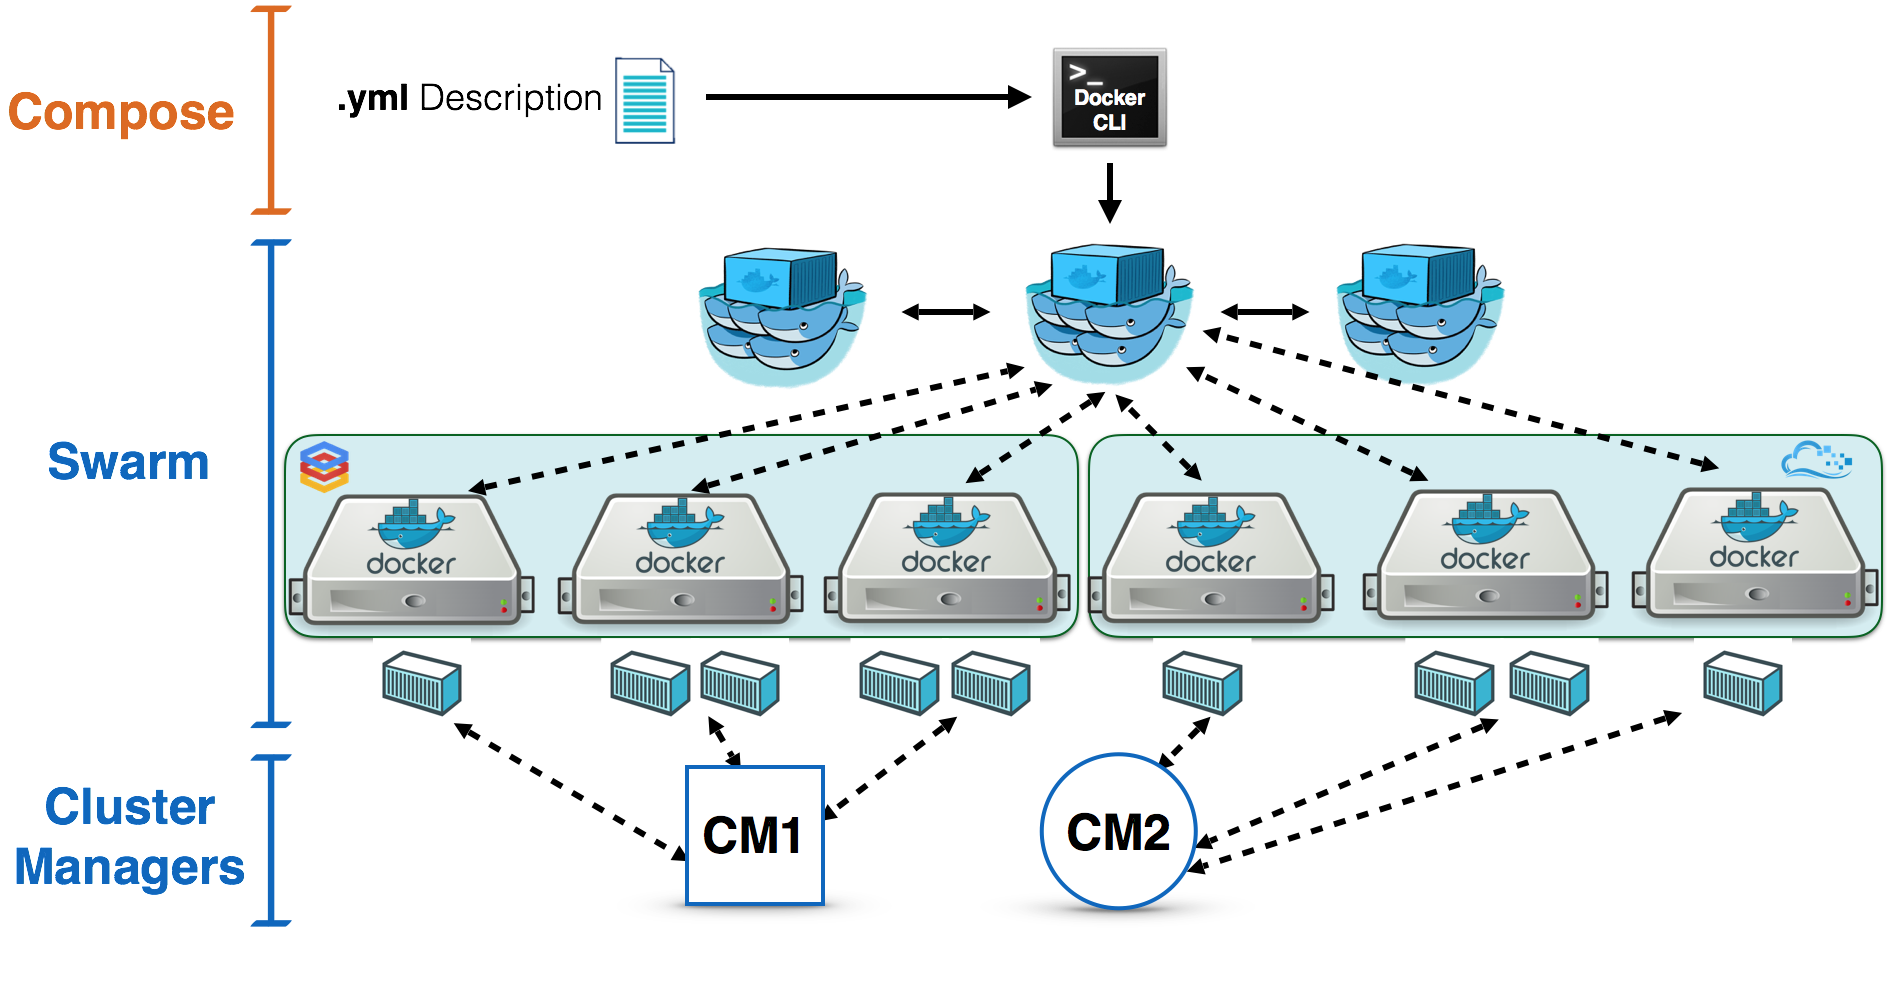
\includegraphics[width=\linewidth]{figures/swarm.png}
	\caption{Docker Swarm architektúra \cite{docker-swarm}}
	\label{fig:swarm}
\end{figure}

\section{Mesos}
A Mesos az Apache szoftvere, mely egy absztrakt környezetet hoz létre CPU, RAM és háttértárral, akár 10.000 node-ig. A Mesos egy nyílt forrású cluster kezelő szoftver. Alkalmazásokat kínál API-kat az erőforrás-kezelésre és az ütemezésre a cluster-en keresztül.  A Mesos rugalmasságot és az elhaló alkalmazások újraindítását biztosítja. Lehetővé teszi a framework-ök számára, hogy ütemezzék és végrehajtják a feladatokat API-n keresztül. A Mesos-architektúra egy master node-ból áll, amely az egyes node-okon futó worker-eket és a worker-eken futó framework-öket kezeli, melyeken a szolgáltatások futnak. Az összes alkalmazásdefiníció egy JSON-fájlban található, amelyet továbbítanak a Mesos / Marathon REST API-hoz.

\section{Kubernetes}
Egy docker rendszerben a definiált konténer egy példánya futtatható a \emph{docker run} utasítással. Kubernetest használva a kube control CLI-on keresztül akár ezer példánya is futtatható ugyanannak az alkalmazásnak.
\begin{lstlisting}[caption={Példa 100 alkalmazás indítására}]
$ kubectl run --replicas=100 wordpress
\end{lstlisting}
A futtatott alkalmazásokat egy másik parancsal felskálázhatjuk.
\begin{lstlisting}[caption={Példa alkalmazás skálázására}]
$ kubectl scale --replicas=200 wordpress
\end{lstlisting}
Tehát egy kihasználtsági emelkedő esetén egyszerűen lefoglalhatunk több erőforrást a felhasználás tekintetében.
A Kubernetes a Docker host programot használja az egyes node-okon alkalmazások futtatásához. Alapvetően konténerekret támogat, azonban nem csak a Docker-t, hanem pl. a Rocket-et és a Cryo-t is.
\subsection{Architektúra}
Egy Kubernetes cluster architektúrája fizikai vagy VM node-okból áll és minden node egy worker (\ref{fig:kubearch}. ábra). Egy node meghibásodása esetén a rajta futó service-t átveszi a többi node. A node-ok között van egy kitüntetett master node, amelyik tárolja a cluster információkat és végzi a manager service-ek processzeit.

\begin{figure}
	\centering
	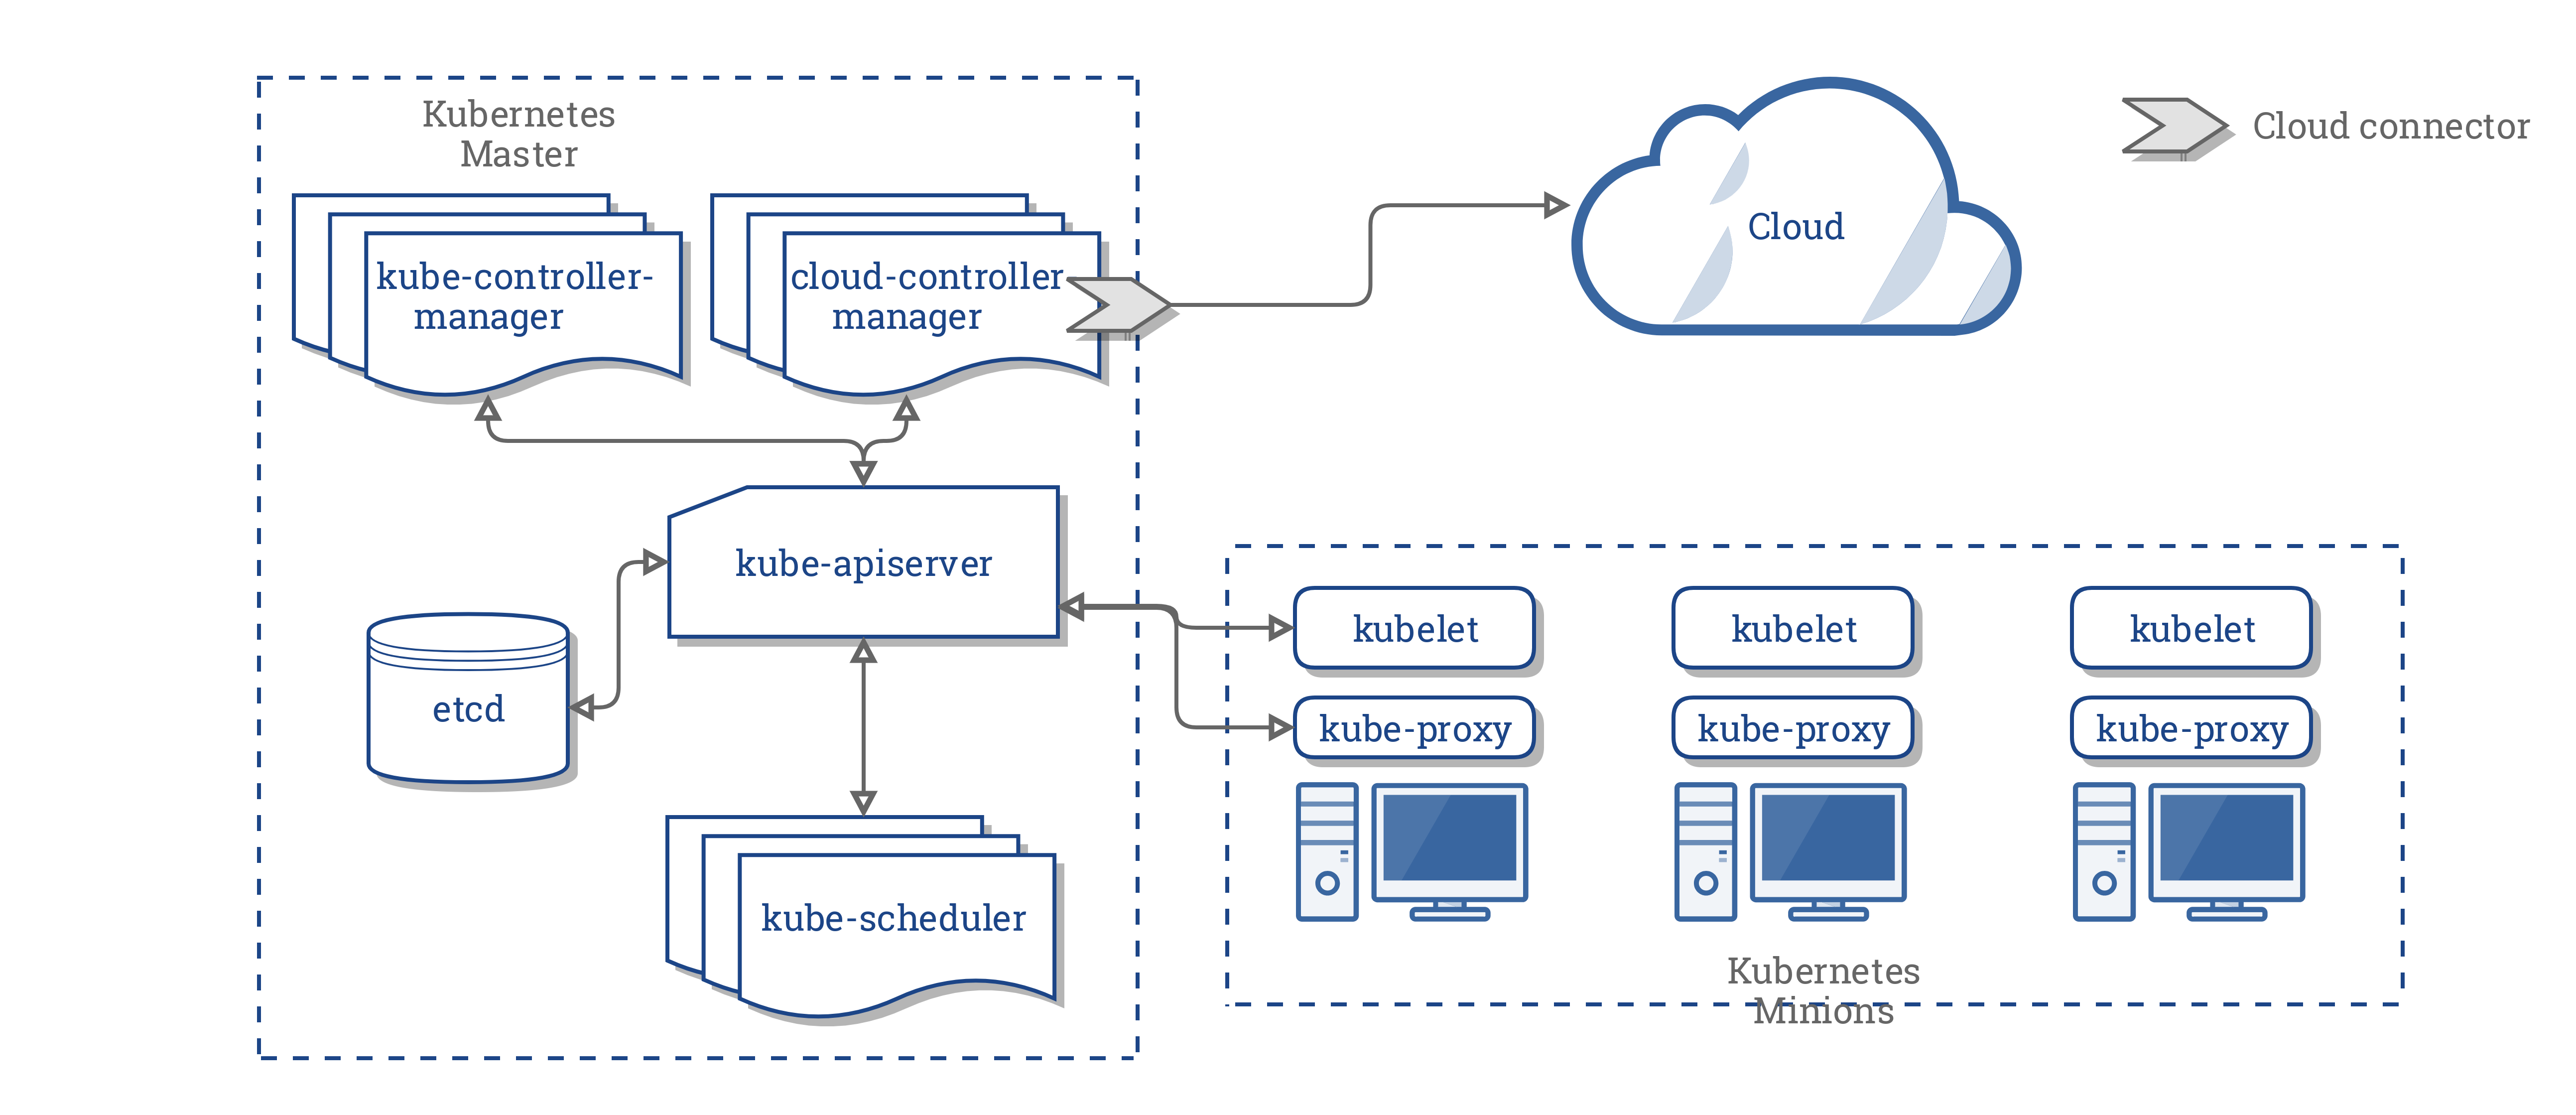
\includegraphics[width=\linewidth]{figures/kube_arch.png}
	\caption{Kubernetes architektúrája \cite{kube-arch}}
	\label{fig:kubearch}
\end{figure}

\subsection{Komponensek}
\paragraphl{API server}
A Kubernetes frontend-jét web UI-t és API-t szolgáltat. Ezzel kommunikál a felhasználó menedzser, CLI-t és a többi UI eszköz is. 
\paragraphl{etcd}
Elosztott kulcsérték tároló, a cluster menedzseléséhez szolgáló információknak.
\paragraphl{Scheduler}
Az elosztott működést valósítja meg a node-okon, minden új feladatot eloszt egy node-hoz.
\paragraphl{Controller}
Figyeli a végpontokat és beavatkozik ha valami tönkremegy.
\paragraphl{Container runtime}
A konténerek keretszoftvere, leggyakoribb esetben a Docker.
\paragraphl{Kubelet}
Ez a service minden node-on fut a cluster-en, a feladata, hogy a node-hoz kiszervezett konténerek fussanak az elvárt módon.
\paragraphl{Kube control}
CLI, amin keresztül az adminisztrátor tud szolgáltatásokat indítani és cluster menedzsment feladatokat ellátni.


\section{Keretrendszer meghatározása}
A nagyszámú robotvezérlés feladatkörében hasonlítom össze a három legelterjedtebb orkesztrációs megoldást.
\begin{center}
	\begin{table}
	\begin{tabular}{ |p{5cm}|p{3cm}|p{3cm}|p{3cm}|  }
		\hline
		\multicolumn{4}{|c|}{Konténer orkesztráció rendszerek} \\
		\hline
		&
		\begin{minipage}{.3\textwidth}
			
\includegraphics[width=3cm]{figures/docker_swarm.png}
		\end{minipage} 
		&
		\begin{minipage}{.3\textwidth}
			
\includegraphics[width=3cm]{figures/mesos.png}
		\end{minipage} 
		&
		\begin{minipage}{.3\textwidth}
			
\includegraphics[width=3cm]{figures/kubernetes.png}
		\end{minipage} 
		 \\
		\hline
		Konténerre optimalizált & \cmark & \xmark & \cmark \\
		Egyszerű telepítés & \cmark & \xmark & \xmark \\
		Szolgáltatás skálázhatóság & \xmark & \xmark & \cmark  \\
		Horizontális skálázhatóság & \cmark & \cmark & \cmark \\
		Vertikális skálázhatóság & \xmark & \cmark & \cmark \\
		Multi-konténer deploy & \cmark & \xmark & \cmark \\
		Minimum node & 1 & 3 masters + slaves & master + 2 slaves \\
		\hline
	\end{tabular}
	\caption{Konténer orkesztrációs rendszerek összehasonlítása}
	\end{table}
\end{center}
A vezérlési rendszerre legoptimálisabb választás a \textbf{Kubernetes}.
\paragraphl{Indoklás}
Egy QoS minőségbiztosított alkalmazás számár nagyon fontos a skálázhatóság és a perzisztencia. Ha kiesik egy node, akkor is fontos, hogy egy kis lassulással is, de stabil maradjon a szolgáltatás. Nagyon jól kezel multi-konténer alkalmazásokat, könnyű a szolgáltatás működése közben új konténereket indítani. A minőségbiztosítási feltételeket a Kubernetes biztosítja a legjobban.
